\chapter{Testes de Verificação e Validação}

\section{Características Gerais}

%\textcolor{red}{Introduzir os principais pontos deste capítulo. Cada teste deve conter explicações completas que garantam sua repetibilidade:
%\begin{itemize}
%    \item Hipóteses levantadas
%    \item Condições de contorno
%    \item Resultados esperados
%    \item Materiais e métodos
%    \item Precisão e acurácia das medidas obtidas.
%\end{itemize}
%}

\subsection{Materiais e métodos}

Para a produção do chassi do projeto, optou-se pela utilização de impressão 3D em conjunto do filamento PETG (Polietileno Tereftalato Glicol) como material principal de impressão. A escolha do filamento sobre outros, como por exemplo o PLA (Poliácido Láctico), se deu pelo filamento possuir alta resistência a impactos e desgaste, e ainda apresentar leveza, baixo custo e facilidade de fabricação.

No que diz respeito ao processo de fabricação, a impressão 3D possibilitou uma simplificação significativa na produção do chassi, não havendo a necessidade de usinagem e desperdício de material, além de permitir a entrega de um produto altamente personalizado e adequado às dimensões e necessidades do projeto.

\subsection{Precisão e acurácia das medidas obtidas}

Para a validação das medidas obtidas, foi seguido um protocolo para coleta de dados, assegurando a acurácia das medidas. As medições dos componentes foram feitas utilizando um paquímetro analógico com incerteza calibrada de $\pm 0,02 mm$, a escolha do instrumento permitiu o monitoramento das dimensões dos encaixes estruturais em relação ao modelo CAD de forma confiável. Para uma maior consistência dos dados obtidos, o protocolo determinou que as medidas do chassi fossem feitas de forma independente por um mesmo operador, após 5 repetições por dimensão foi verificado o desvio padrão amostral, valores de desvio próximo a zero confirmaram uma alta precisão em suas medidas.

\section{Testes da estrutura}

A montagem do chassi impresso em 3D com as abraçadeiras foi feita fielmente ao modelo CAD, já colorido e mostrando só as peças relevantes ao caso (Figura \ref{fig:rendcolorida}).

\begin{figure}[H]
    \centering
    \begin{subfigure}{0.48\linewidth}
        \centering
        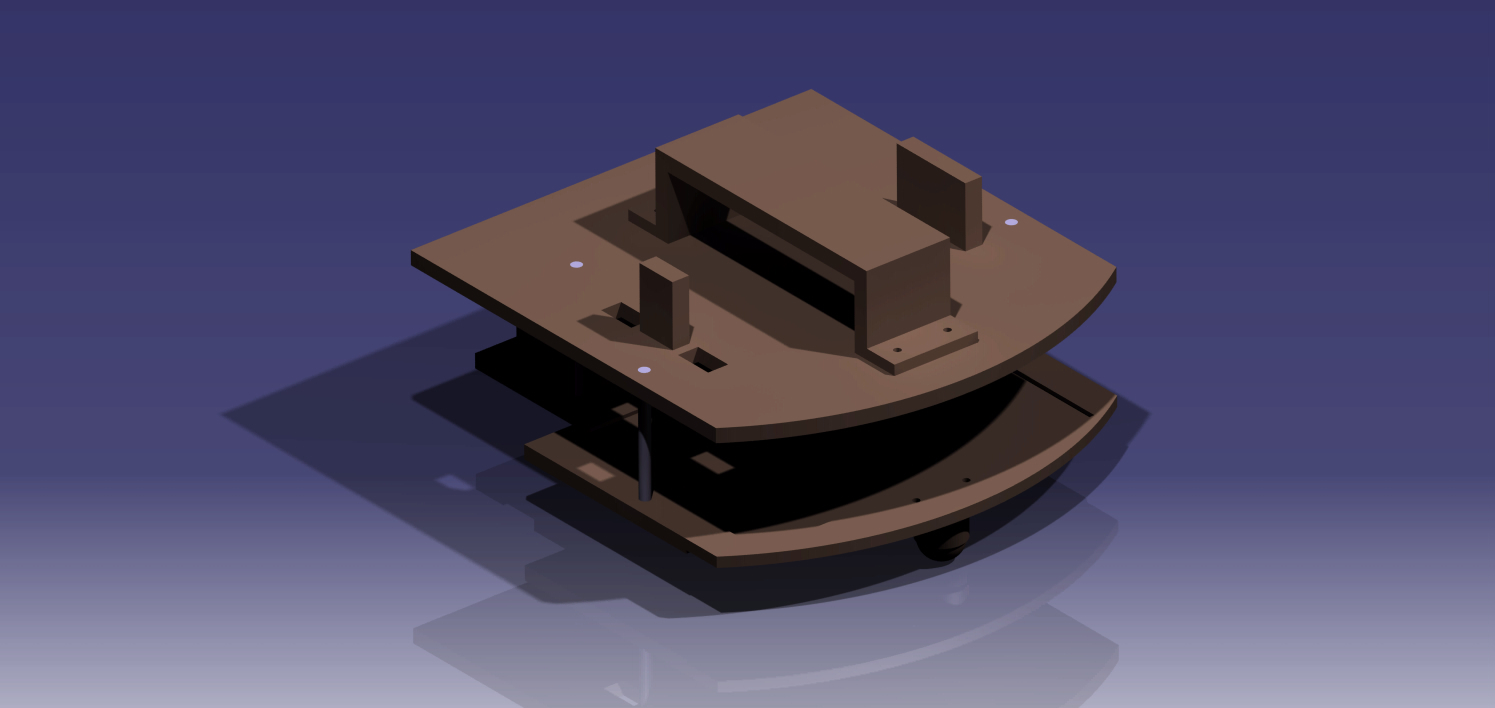
\includegraphics[width=\linewidth]{figuras/fotocadfinal.jpg}
    \end{subfigure}
    \hfill
    \begin{subfigure}{0.48\linewidth}
        \centering
        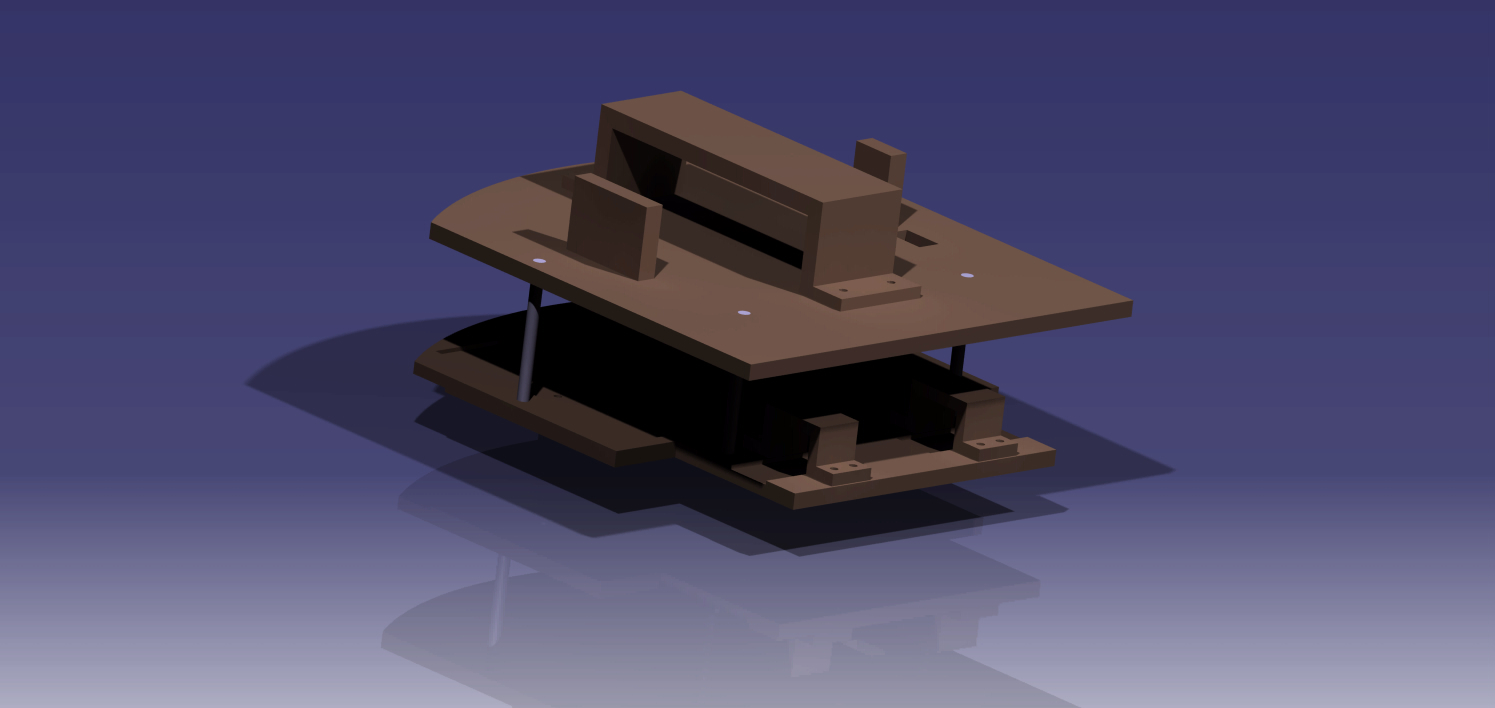
\includegraphics[width=\linewidth]{figuras/fotocadfinal2.jpg}
    \end{subfigure}
    \caption{Renderização colorida das peças impressas, em duas vistas.}
    \label{fig:rendcolorida}
\end{figure}

A Figura \ref{fig:insertos_parafusacao} mostra os dois níveis do chassi com os insertos de latão ao lado, prontos para a junção, e em seguida já com as abraçadeiras, prontos para a parafusação e a inserção dos separadores de nível.

\begin{figure}[H]
    \centering
    \begin{subfigure}{0.48\linewidth}
        \centering
        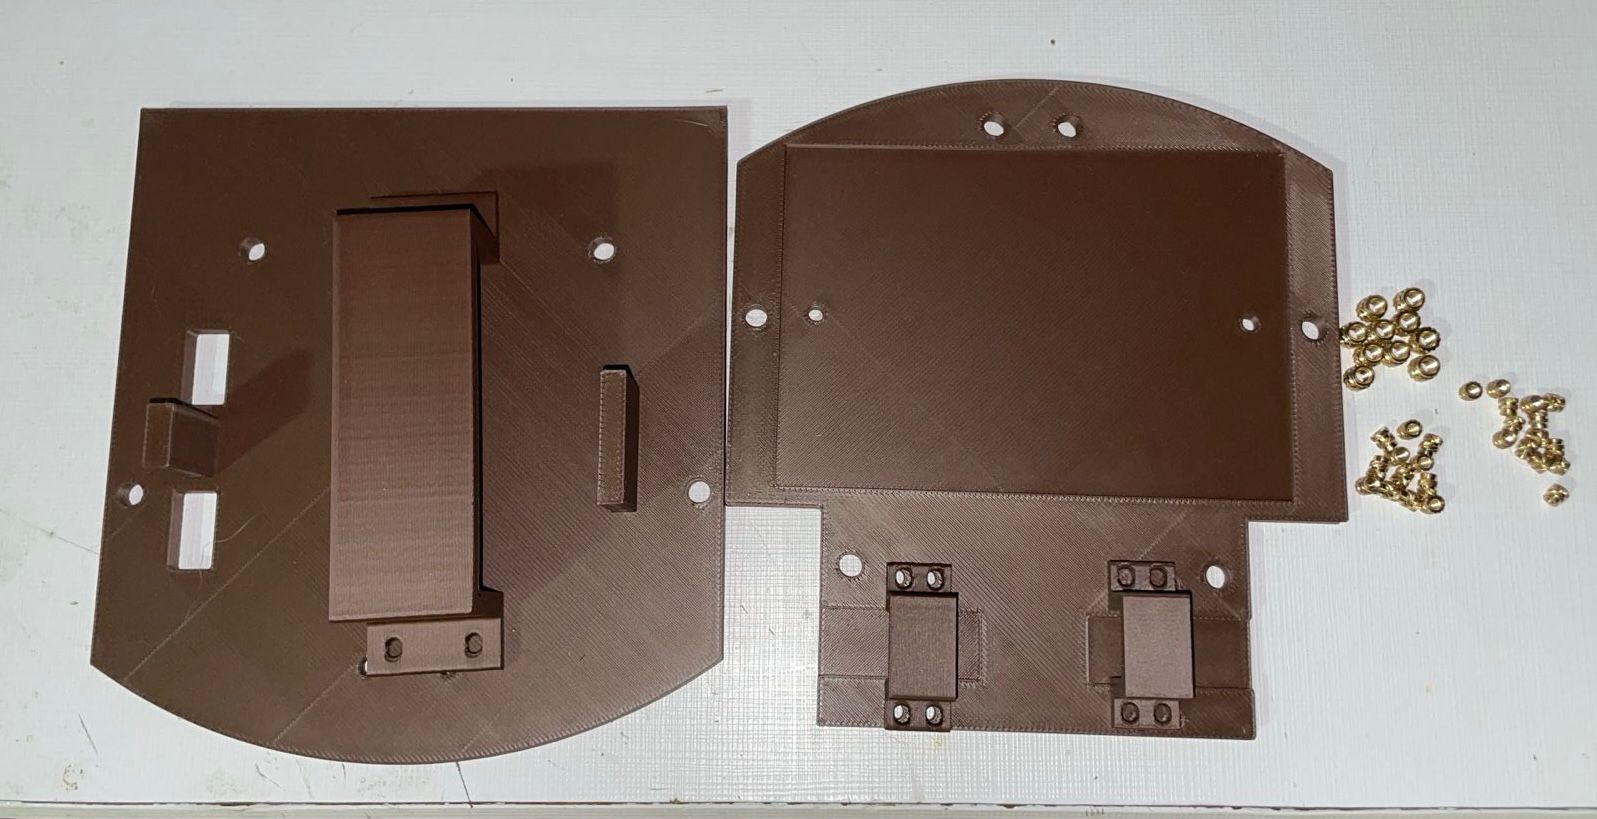
\includegraphics[width=\linewidth]{figuras/fotomontagem1.jpeg}
    \end{subfigure}
    \hfill
    \begin{subfigure}{0.48\linewidth}
        \centering
        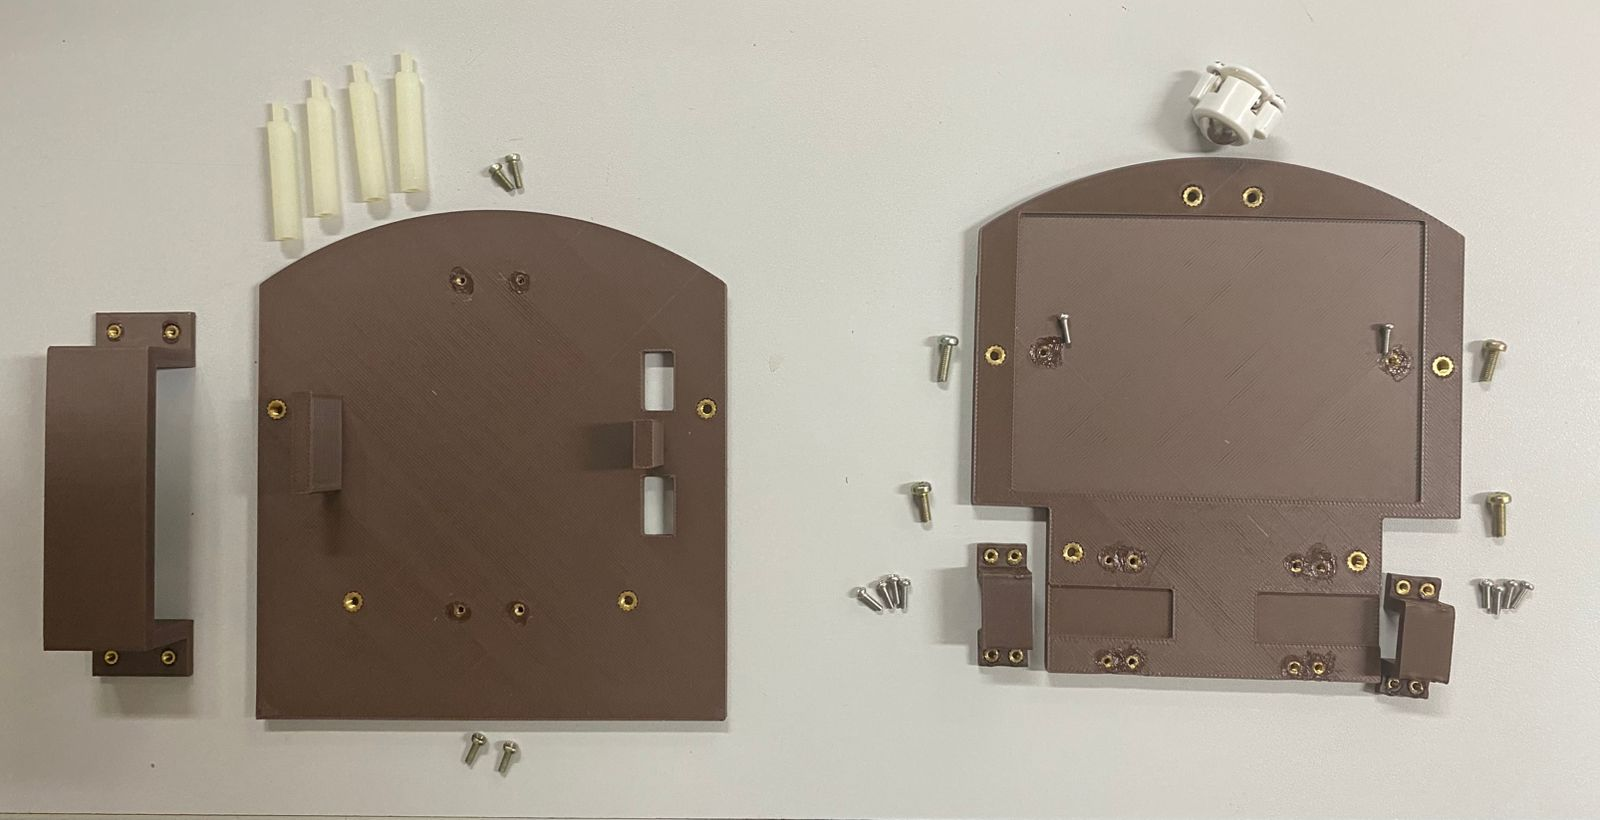
\includegraphics[width=\linewidth]{figuras/fotomontagem2.jpeg}
    \end{subfigure}
    \caption{Preparação para junção dos insertos de latão (esquerda) e componentes da parafusação (direita).}
    \label{fig:insertos_parafusacao}
\end{figure}

A Figura \ref{fig:montagem_final} mostra a carcaça do micromouse montada e parafusada, com os níveis separados pelos espaçadores de nylon e as abraçadeiras fixadas, em duas vistas.

\begin{figure}[H]
    \centering
    \begin{subfigure}{0.48\linewidth}
        \centering
        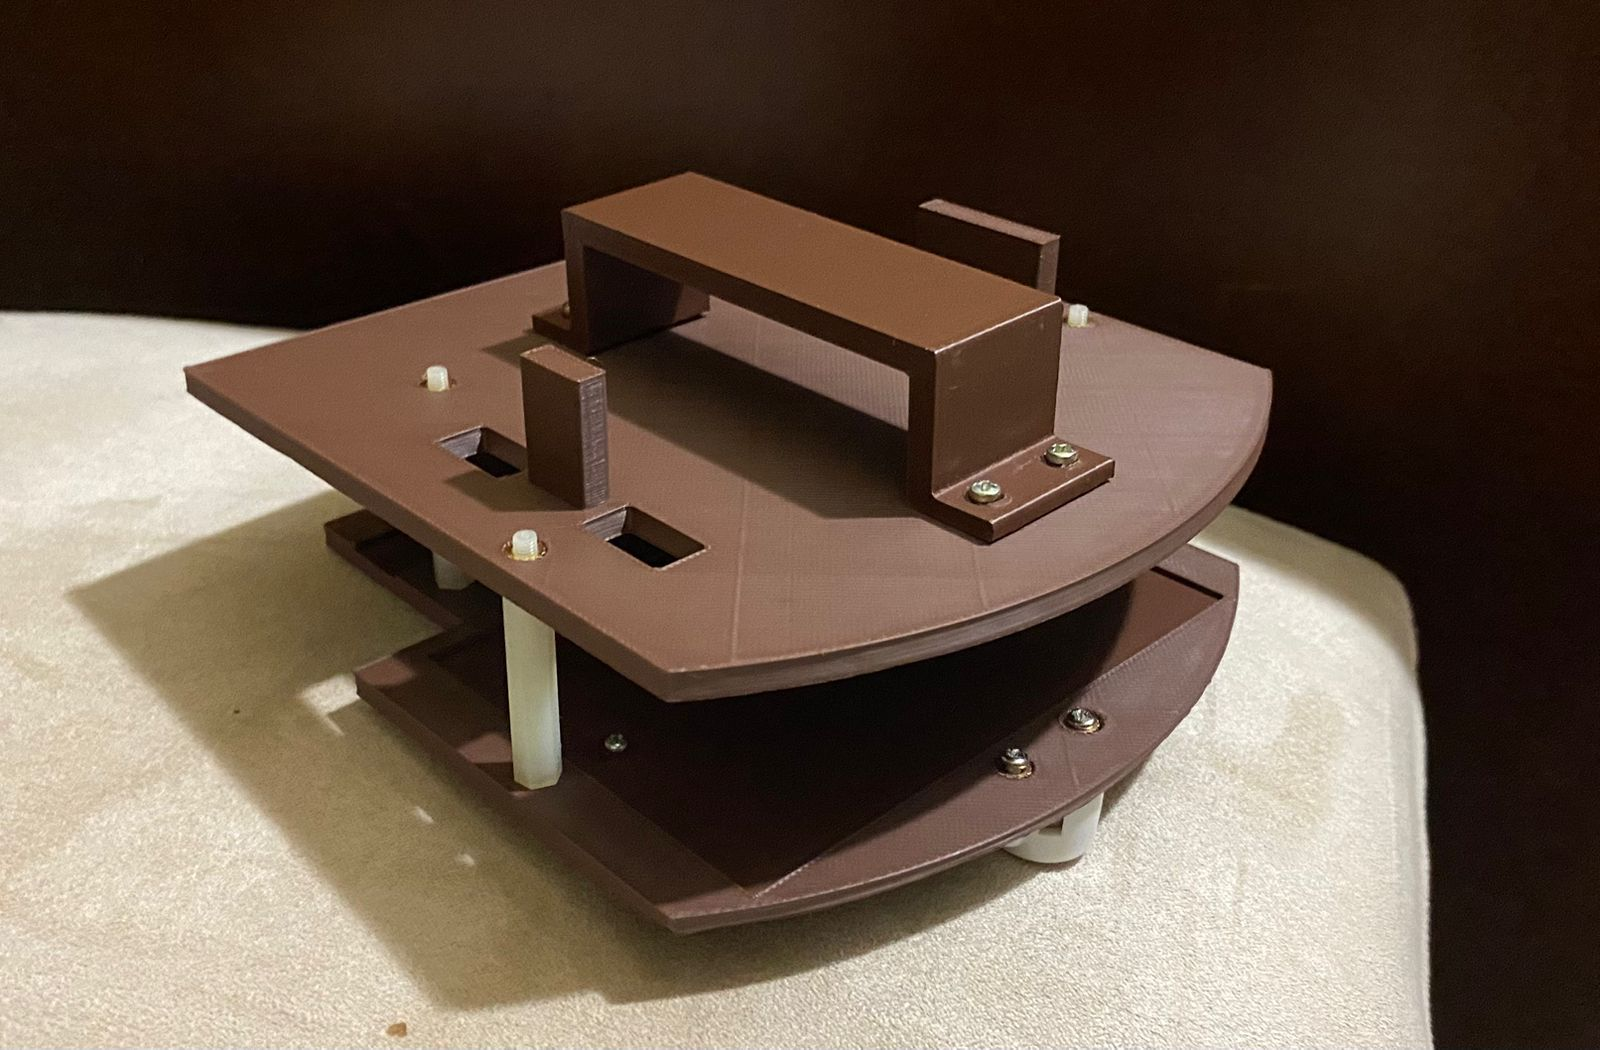
\includegraphics[width=\linewidth]{figuras/fotomontagem3.jpeg}
    \end{subfigure}
    \hfill
    \begin{subfigure}{0.48\linewidth}
        \centering
        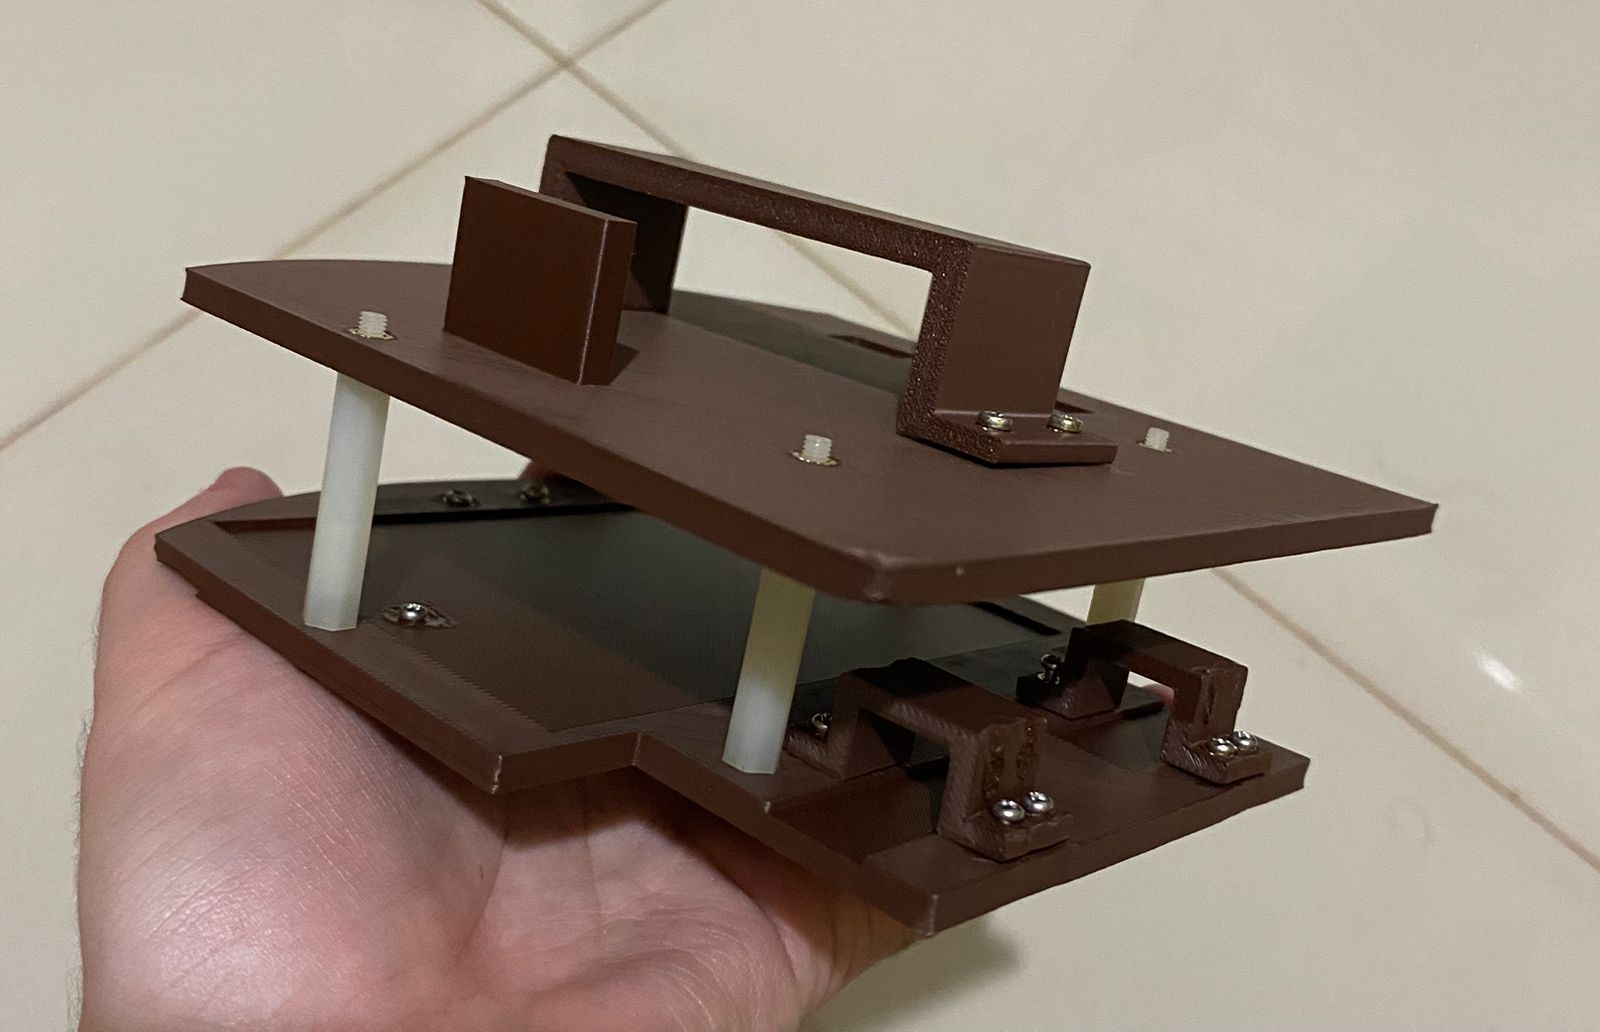
\includegraphics[width=\linewidth]{figuras/fotomontagem4.jpeg}
    \end{subfigure}
    \caption{Carcaça do micromouse montada e parafusada, em duas vistas.}
    \label{fig:montagem_final}
\end{figure}

\section{Testes de \textit{hardware}}

%\textcolor{red}{Apresentar com detalhes os testes feitos para conferir se os objetivos do \textit{hardware} foram atendidos, incluindo:}
%
%\begin{enumerate}
%    \item \textcolor{red}{Processamento (Arduino, ESP32 etc):}
%    \begin{itemize}
%        \item \textcolor{red}{Definir interface de desenvolvimento;}
%        \item \textcolor{red}{Rodar exemplo mínimo.}
%    \end{itemize}
%    \item \textcolor{red}{Sensores (temperatura, pressão, posição, velocidade etc.):}
%    \begin{itemize}
%        \item \textcolor{red}{Realizar leitura básica de dados;}
%        \item \textcolor{red}{Validar/calibrar leituras;}
%        \item \textcolor{red}{Definir taxas de amostragem e quantidade de dados para transmissão e/ou armazenamento;}
%        \item \textcolor{red}{Validar taxas definidas e quantidade de dados;}
%        \item \textcolor{red}{Realizar processamento básico de dados (\textit{thresholding}, filtro média-móvel etc.).}
%    \end{itemize}
%    \item \textcolor{red}{Armazenamento (memória interna, cartão SD, pendrive etc.):}
%    \begin{itemize}
%        \item \textcolor{red}{Armazenar dados básicos;}
%        \item \textcolor{red}{Armazenar e validar dados de sensores.}
%    \end{itemize}
%    \item \textcolor{red}{Atuadores (Motores DC, relés, LEDs etc.):}
%    \begin{itemize}
%        \item \textcolor{red}{Realizar acionamentos básicos;}
%        \item \textcolor{red}{Realizar acionamentos com base em dados de sensores;}
%        \item \textcolor{red}{Realizar processamento básico de dados (PWM etc.).}
%    \end{itemize}
%    \item \textcolor{red}{Comunicações (UART, I2C, SPI, USB, WiFi, Bluetooth etc.):}
%    \begin{itemize}
%        \item \textcolor{red}{Transmissão básica de dados;}
%        \item \textcolor{red}{Transmissão de dados de sensores dentro da taxa de amostragem.}
%    \end{itemize}
%\end{enumerate}

Os testes de sensores foram realizados nos laboratórios NEI 1 e NEI 2 da FCTE. Em cada caso, o sensor foi montado em protoboard junto ao Raspberry Pi Pico W, conectado por jumpers conforme a Tabela~\ref{tab:pinagem_testes}, e um firmware de teste em C/C++ foi gravado via USB para inicializar o sensor e imprimir as leituras no monitor serial, permitindo verificar o funcionamento por observação direta.

\begin{table}[H]
\centering
\caption{Conexões utilizadas nos testes de sensores}
\label{tab:pinagem_testes}
\begin{tabular}{|l|l|l|}
\hline
\textbf{Sensor} & \textbf{Sinais} & \textbf{Pinos físicos (Pico W)} \\
\hline
MPU-6050 & SDA, SCL, VCC, GND, AD0 & 6, 7, 36 (3V3), 38 (GND), 38 (GND) \\
\hline
HC-SR04 & Trig, Echo, VCC, GND & 20, 19, 36 (3V3), 38 (GND) \\
\hline
VL53L0X (esq. / dir.) & SDA, SCL, VIN, GND & 6/19, 7/20, 36 (3V3), 38 (GND) \\
\hline
\end{tabular}
\end{table}

\subsection{Teste Sensor Giroscópio MPU-6050}

O eixo Z (\textit{yaw}), perpendicular ao chão, é o principal usado para o giro do robô; X (\textit{roll}) e Y (\textit{pitch}) correspondem às inclinações lateral e frontal/traseira. Após a calibração automática, indicada por dois piscares do LED, a protoboard foi rotacionada manualmente pelas quatro direções cardinais, e o monitor serial (porta COM3) confirmou a leitura correta da orientação (\textit{north/east/south/west}) em cada posição.

\begin{figure}[H]
    \centering
    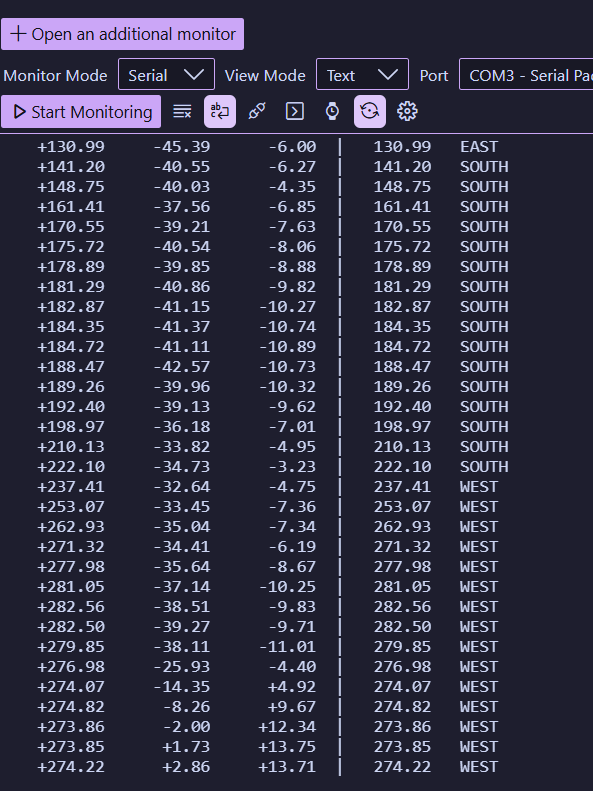
\includegraphics[width=0.35\linewidth]{figuras/teste_mpu6050.png}
    \caption{Monitor serial com visualização de dados fornecidos pelo sensor mpu6050.}
    \label{fig:teste Sensor mpu6050}
\end{figure}

\subsection{Teste Sensor Ultrassônico HC-SR04}

A medição baseia-se no tempo entre a emissão de um pulso ultrassônico pelo pino Trig e o retorno do eco pelo pino Echo, convertido em distância pela velocidade do som no ar. Um objeto plano foi posicionado a distâncias conhecidas, previamente medidas com régua, e as leituras exibidas no monitor serial (porta COM5) confirmaram a consistência e a precisão do sensor.

\begin{figure}[H]
    \centering
    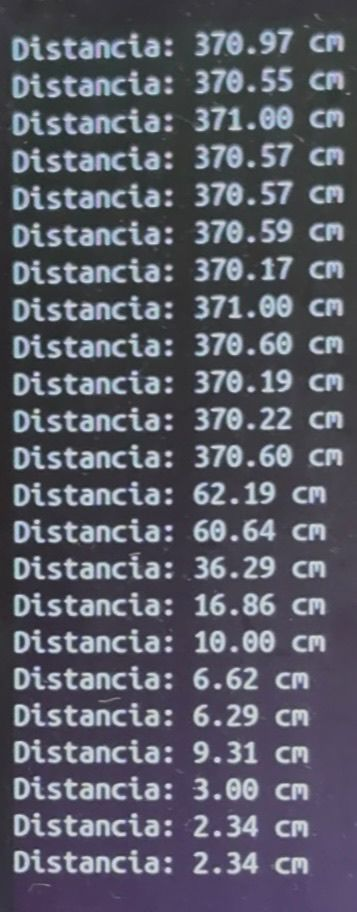
\includegraphics[width=0.35\linewidth]{figuras/teste_hcsr04.png}
    \caption{Monitor serial com visualização de dados fornecidos pelo sensor hc-sr04.}
    \label{fig:teste Sensor hcsr04}
\end{figure}

\subsection{Teste Sensor Infravermelho VL53L0X}

Os dois sensores VL53L0X (esquerdo e direito) foram conectados a barramentos I²C independentes do Pico W. Após a inicialização sequencial de ambos, objetos foram aproximados e afastados manualmente em frente a cada sensor, individualmente e em conjunto, com as distâncias em milímetros exibidas em tempo real no monitor serial (porta COM5), confirmando a leitura simultânea e independente dos dois sensores.

\begin{figure}[H]
    \centering
    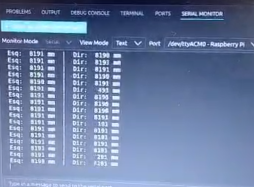
\includegraphics[width=0.35\linewidth]{figuras/teste_vl53l0x.png}
    \caption{Monitor serial com visualização de dados fornecidos pelo sensor vl53l0x.}
\end{figure}


%\textcolor{red}{Apresentar com detalhes os testes feitos para conferir se as demandas energéticas do projeto foram atendidas.}

\section{Testes de Consumo Energético}

\subsection{Caracterização da Fonte de Alimentação}

O sistema de alimentação do micromouse é composto por duas baterias de íon-lítio de 3,7 V e 4400 mAh conectadas em série, resultando em tensão nominal de 7,4 V e capacidade de 4400 mAh.

A energia total armazenada no conjunto é dada por:

\begin{equation}
E = V \times C
\end{equation}

\begin{equation}
E = 7,4 \times 4,4 = 32,56 { Wh}
\end{equation}

Considerando uma eficiência prática de 85\%, referente às perdas no regulador step-down necessário para alimentação da Raspberry Pi Pico W e demais componentes de 3,3 V e 5 V, a energia efetivamente disponível ao sistema é:

\begin{equation}
E_{disp} = 32,56 \times 0,85 = 27,68 { Wh}
\end{equation}

equivalente a uma carga útil aproximada de 3740 mAh referenciada a 7,4 V.

\subsection{Levantamento do Consumo por Componente}

A Tabela \ref{tab:consumo_componentes} apresenta o consumo estimado de cada componente do micromouse, com base nos datasheets dos fabricantes e em referências técnicas para componentes similares. Os valores de corrente são referenciados à tensão de operação de cada dispositivo após regulação.

\begin{table}[H]
\centering
\caption{Consumo estimado dos componentes do micromouse}
\label{tab:consumo_componentes}
\resizebox{\textwidth}{!}{
\begin{tabular}{|l|c|c|c|p{5cm}|}
\hline
\textbf{Componente} & \textbf{Qtd.} & \textbf{Corrente Unitária (mA)} & \textbf{Corrente Total (mA)} & \textbf{Observações} \\
\hline
Raspberry Pi Pico W & 1 & 43 & 43 & Operação ativa, Wi-Fi desabilitado \\
\hline
Raspberry Pi Pico W (Wi-Fi ativo) & 1 & $\sim$100 & $\sim$100 & Durante transmissão Wi-Fi \\
\hline
Motor GA12-N20 & 2 & 150--200 & 350 & Operação nominal a aproximadamente 60\% da tensão via PWM \\
\hline
Driver TB6612FNG & 1 & 2--5 & 4 & Consumo estático do CI \\
\hline
Sensor VL53L0X (ToF) & 2 & 19--20 & 38 & Modo de medição contínua \\
\hline
Sensor HC-SR04 & 1 & 20 & 20 & Alimentado via VBUS (5 V) \\
\hline
Sensor MPU-6050 & 1 & 3,5--5 & 4 & Giroscópio e acelerômetro ativos \\
\hline
Módulo sensor de corrente (5 A) & 1 & $\sim$12 & 12 & Baseado em módulos ACS712 similares \\
\hline
Módulo sensor de tensão (0--25 V) & 1 & $\sim$1,5 & 1,5 & Divisor resistivo com buffer \\
\hline
LED vermelho & 1 & 2 & 2 & Com resistor limitador de 1 k$\Omega$ a 3,3 V \\
\hline
Resistores (1 k$\Omega$ e 2,2 k$\Omega$) & -- & $<$0,5 & 0,5 & Perdas desprezíveis \\
\hline
\textbf{Total (Wi-Fi off)} & & & \textbf{$\sim$475} & Regime normal de operação \\
\hline
\textbf{Total (Wi-Fi ativo)} & & & \textbf{$\sim$532} & Com transmissão contínua \\
\hline
\end{tabular}
}
\end{table}

\textbf{Nota:} Os valores dos motores GA12-N20 referem-se à condição de cruzeiro com ciclo PWM reduzido. Em partida ou travamento, o pico de corrente pode atingir entre 500 mA e 1000 mA por motor, condição transitória que deve ser considerada no dimensionamento das proteções do driver.

\subsection{Distribuição do Consumo Energético}

A análise percentual do consumo em regime normal ($\sim$475 mA) revela a distribuição apresentada na Tabela \ref{tab:distribuicao_consumo}.

\begin{table}[H]
\centering
\caption{Distribuição percentual do consumo energético}
\label{tab:distribuicao_consumo}
\begin{tabular}{|l|c|c|}
\hline
\textbf{Grupo de Componentes} & \textbf{Corrente (mA)} & \textbf{Participação (\%)} \\
\hline
Motores GA12-N20 (2x) & 350 & 73,7 \\
\hline
Raspberry Pi Pico W & 43 & 9,1 \\
\hline
Sensores (VL53L0X, HC-SR04 e MPU-6050) & 62 & 13,1 \\
\hline
Driver e módulos auxiliares & 17,5 & 3,7 \\
\hline
LED e resistores & 2,5 & 0,5 \\
\hline
\end{tabular}
\end{table}

Os motores representam isoladamente a maior parcela do consumo total, resultado esperado em plataformas de robótica móvel, onde os atuadores dominam o orçamento energético. Essa característica reforça a importância do controle eficiente de velocidade via PWM, que reduz a corrente média consumida pelos motores ao longo do percurso no labirinto.

\subsection{Análise da Autonomia do Sistema}

Com base nos valores levantados, calculou-se a autonomia do sistema em três cenários de operação:

\begin{itemize}
    \item \textbf{Cenário 1:} Operação em labirinto (Wi-Fi desabilitado e motores em regime).
    \item \textbf{Cenário 2:} Operação com monitoramento via Wi-Fi (transmissão contínua).
    \item \textbf{Cenário 3:} Pico de demanda (partida simultânea dos dois motores).
\end{itemize}

A corrente de pico estimada é de aproximadamente:

\begin{equation}
I_{pico} \approx 1600 { mA}
\end{equation}

correspondente a:

\begin{equation}
I_{pico} \approx (2 \times 500) + 600
\end{equation}

onde os motores contribuem com aproximadamente 1000 mA e os demais componentes com cerca de 600 mA.

Este terceiro cenário representa uma condição transitória e não o regime contínuo de operação do robô, sendo apresentado apenas para fins de dimensionamento das proteções elétricas.

\subsection{Considerações sobre a Viabilidade Energética}

Os resultados indicam que o sistema possui autonomia energética suficiente para aplicações de micromouse, com tempo de operação estimado entre 7 e 8 horas.

Como o pack de baterias opera em 7,4 V, é necessário utilizar um regulador step-down para alimentar a Raspberry Pi Pico W com segurança, enquanto os motores devem ser controlados por PWM para operar dentro de sua faixa nominal.

Além disso, recomenda-se o monitoramento contínuo da tensão das baterias por meio do sensor integrado, com implementação de proteção por subtensão abaixo de 6,0 V, evitando descargas profundas e aumentando a vida útil das células.

\section{Testes de \textit{software}}

Como o \textit{hardware} do micromouse ainda está em fase de montagem e integração, os testes de \textit{software} foram realizados com um simulador de \textit{firmware} desenvolvido pela própria equipe, que reproduz o comportamento esperado do robô real: percorre o labirinto em ziguezague, calcula as paredes de cada célula visitada e publica pacotes MQTT no mesmo formato e protocolo que o \textit{firmware} definitivo utilizará, validando todo o pipeline de dados -- do envio até a exibição no \textit{dashboard} -- antes mesmo de o robô estar pronto.

\subsection{Envio de telemetria}

Na integração real, quem publica as mensagens via MQTT será o Raspberry Pi Pico W embarcado no robô; nos testes, esse papel foi assumido pelo simulador. A cada passo simulado, o sistema publica um pacote JSON no tópico \texttt{micromouse/<id>/telemetria} com QoS~1, contendo posição, orientação, paredes da célula, velocidade, bateria e tensão -- decrementando a bateria gradualmente (0,4\% por passo) e variando a velocidade entre 0,25 e 0,35~m/s para aproximar uma corrida real. No \textit{backend}, um processo dedicado (\texttt{mqtt\_subscribe}) escuta esses tópicos e enfileira uma tarefa assíncrona no Celery para persistir os dados sem travar o loop de recepção.

\subsection{Exibição de telemetria}

O \textit{backend} usa \textit{Server-Sent Events} em vez de \textit{polling}: após processar cada pacote, publica um \textit{snapshot} atualizado em um canal do Redis, que o \textit{frontend} consome por conexão aberta, sem atraso perceptível. A Figura~\ref{fig:dashboard_telemetria} mostra o \textit{dashboard} principal em dois momentos da corrida simulada, exibindo em tempo real velocidade média, tempo decorrido, bateria, tensão, células exploradas no labirinto 16$\times$16 e os três sensores de distância.

\begin{figure}[H]
    \centering
    \begin{subfigure}{0.48\linewidth}
        \centering
        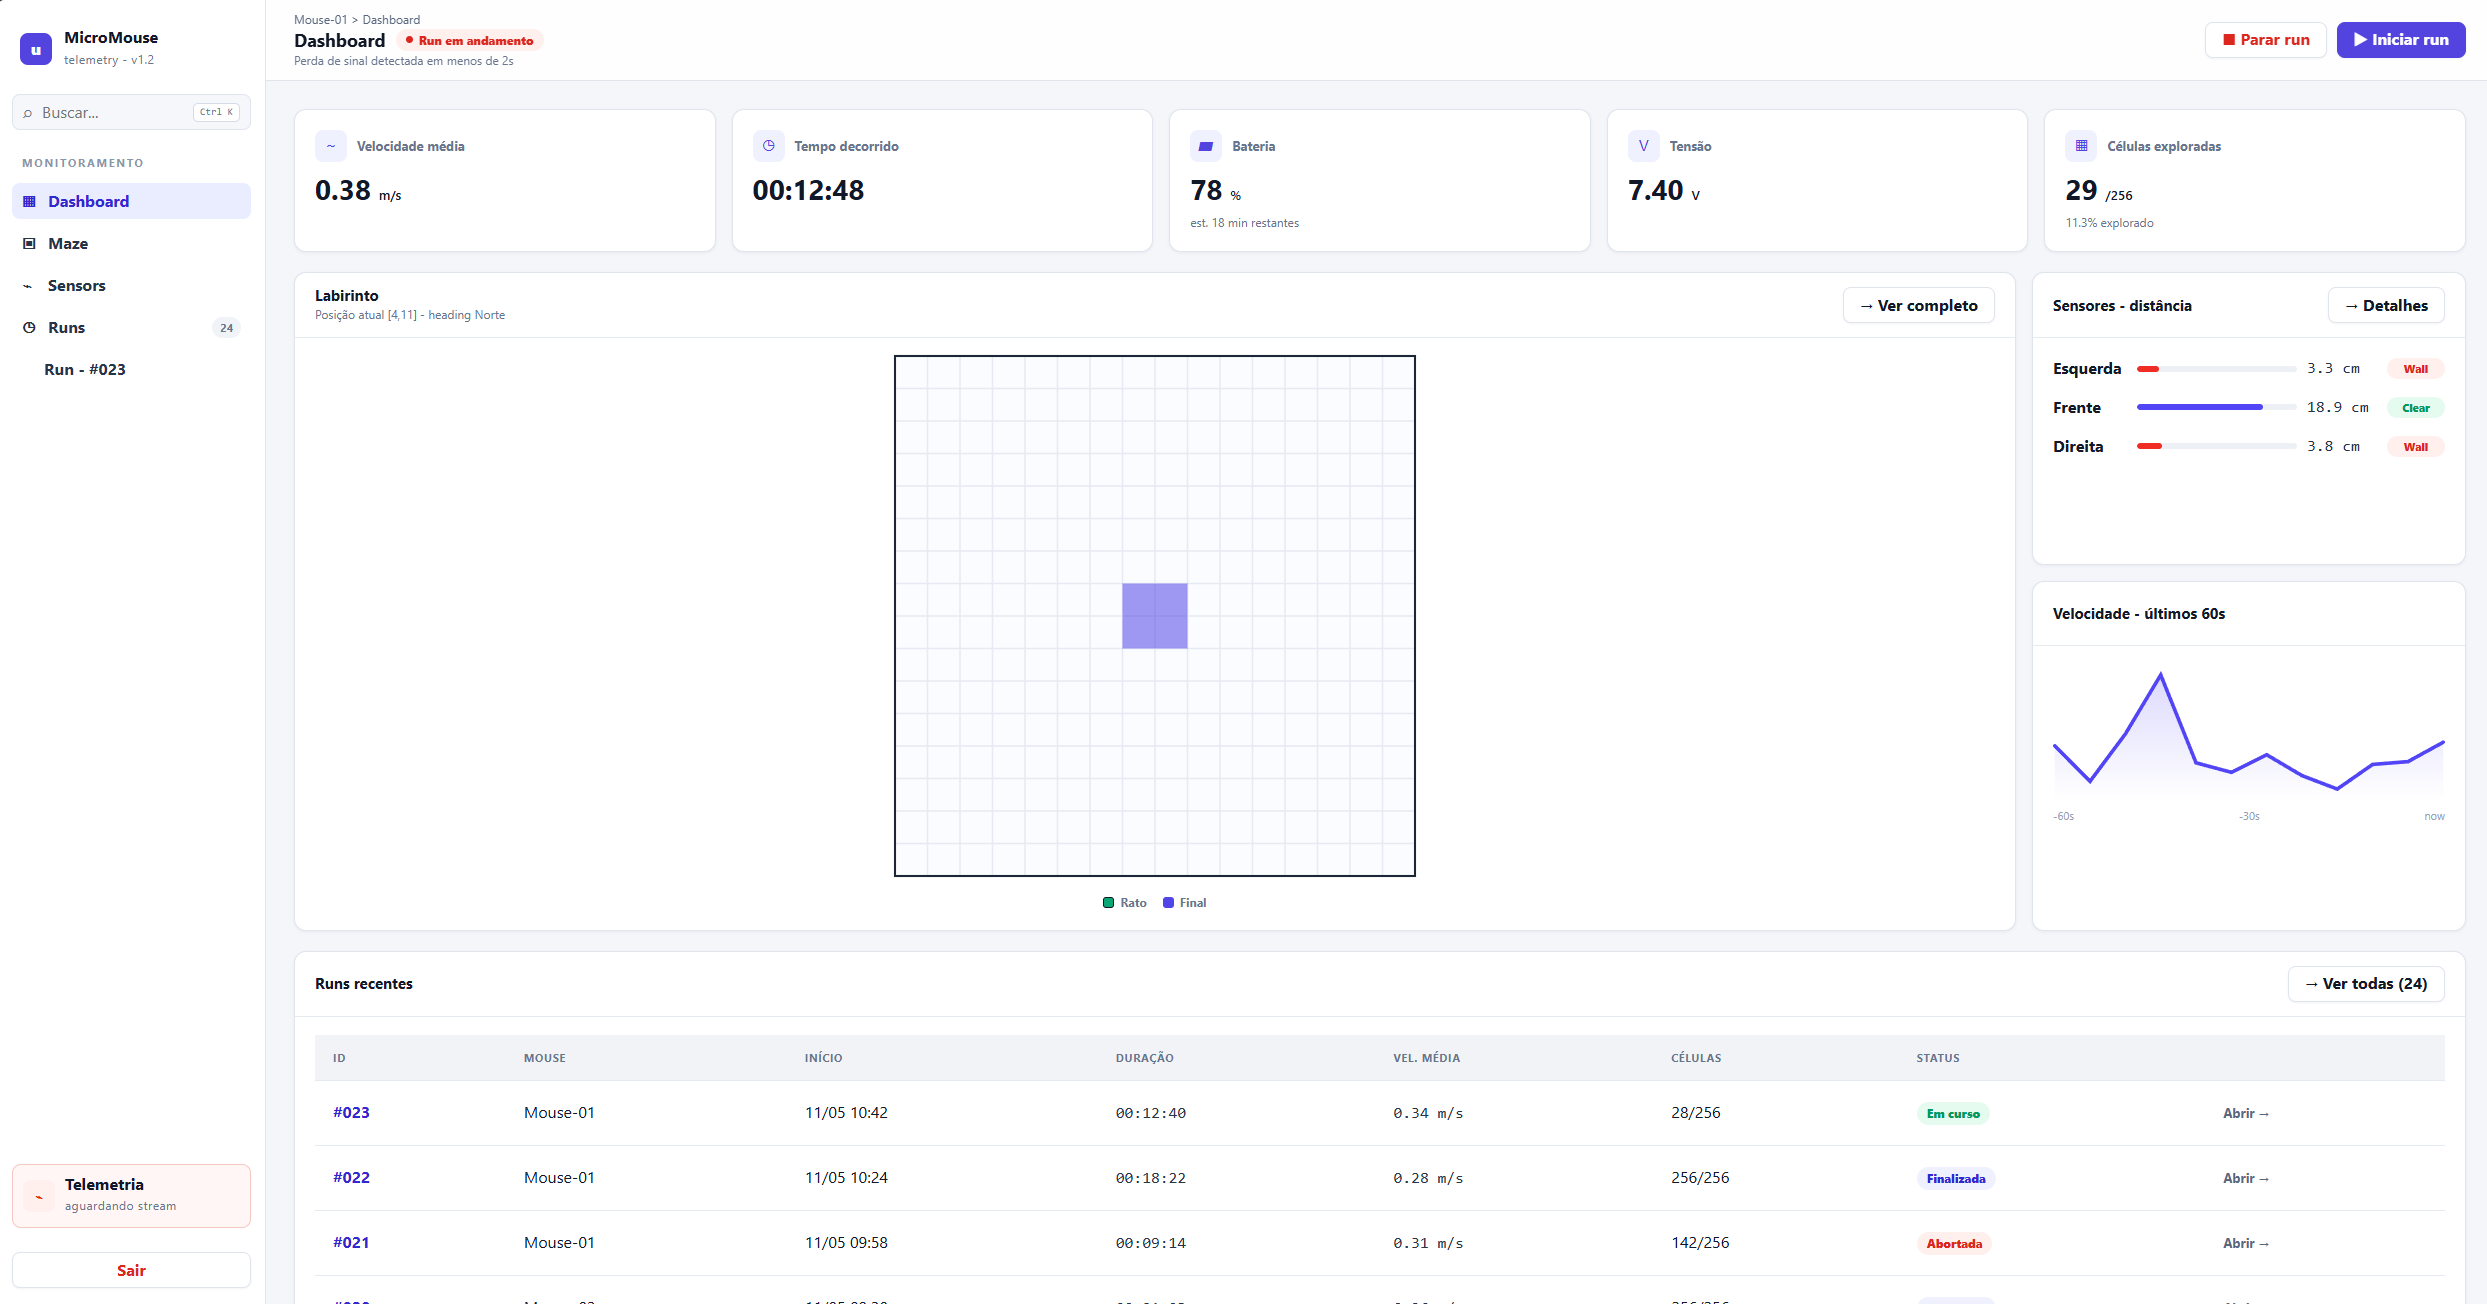
\includegraphics[width=\linewidth]{figuras/dashboard_telemetria_inicio.png}
        \caption{Início: 29 células (11,3\%), 0,38~m/s, bateria 78\%, 7,40~V.}
    \end{subfigure}
    \hfill
    \begin{subfigure}{0.48\linewidth}
        \centering
        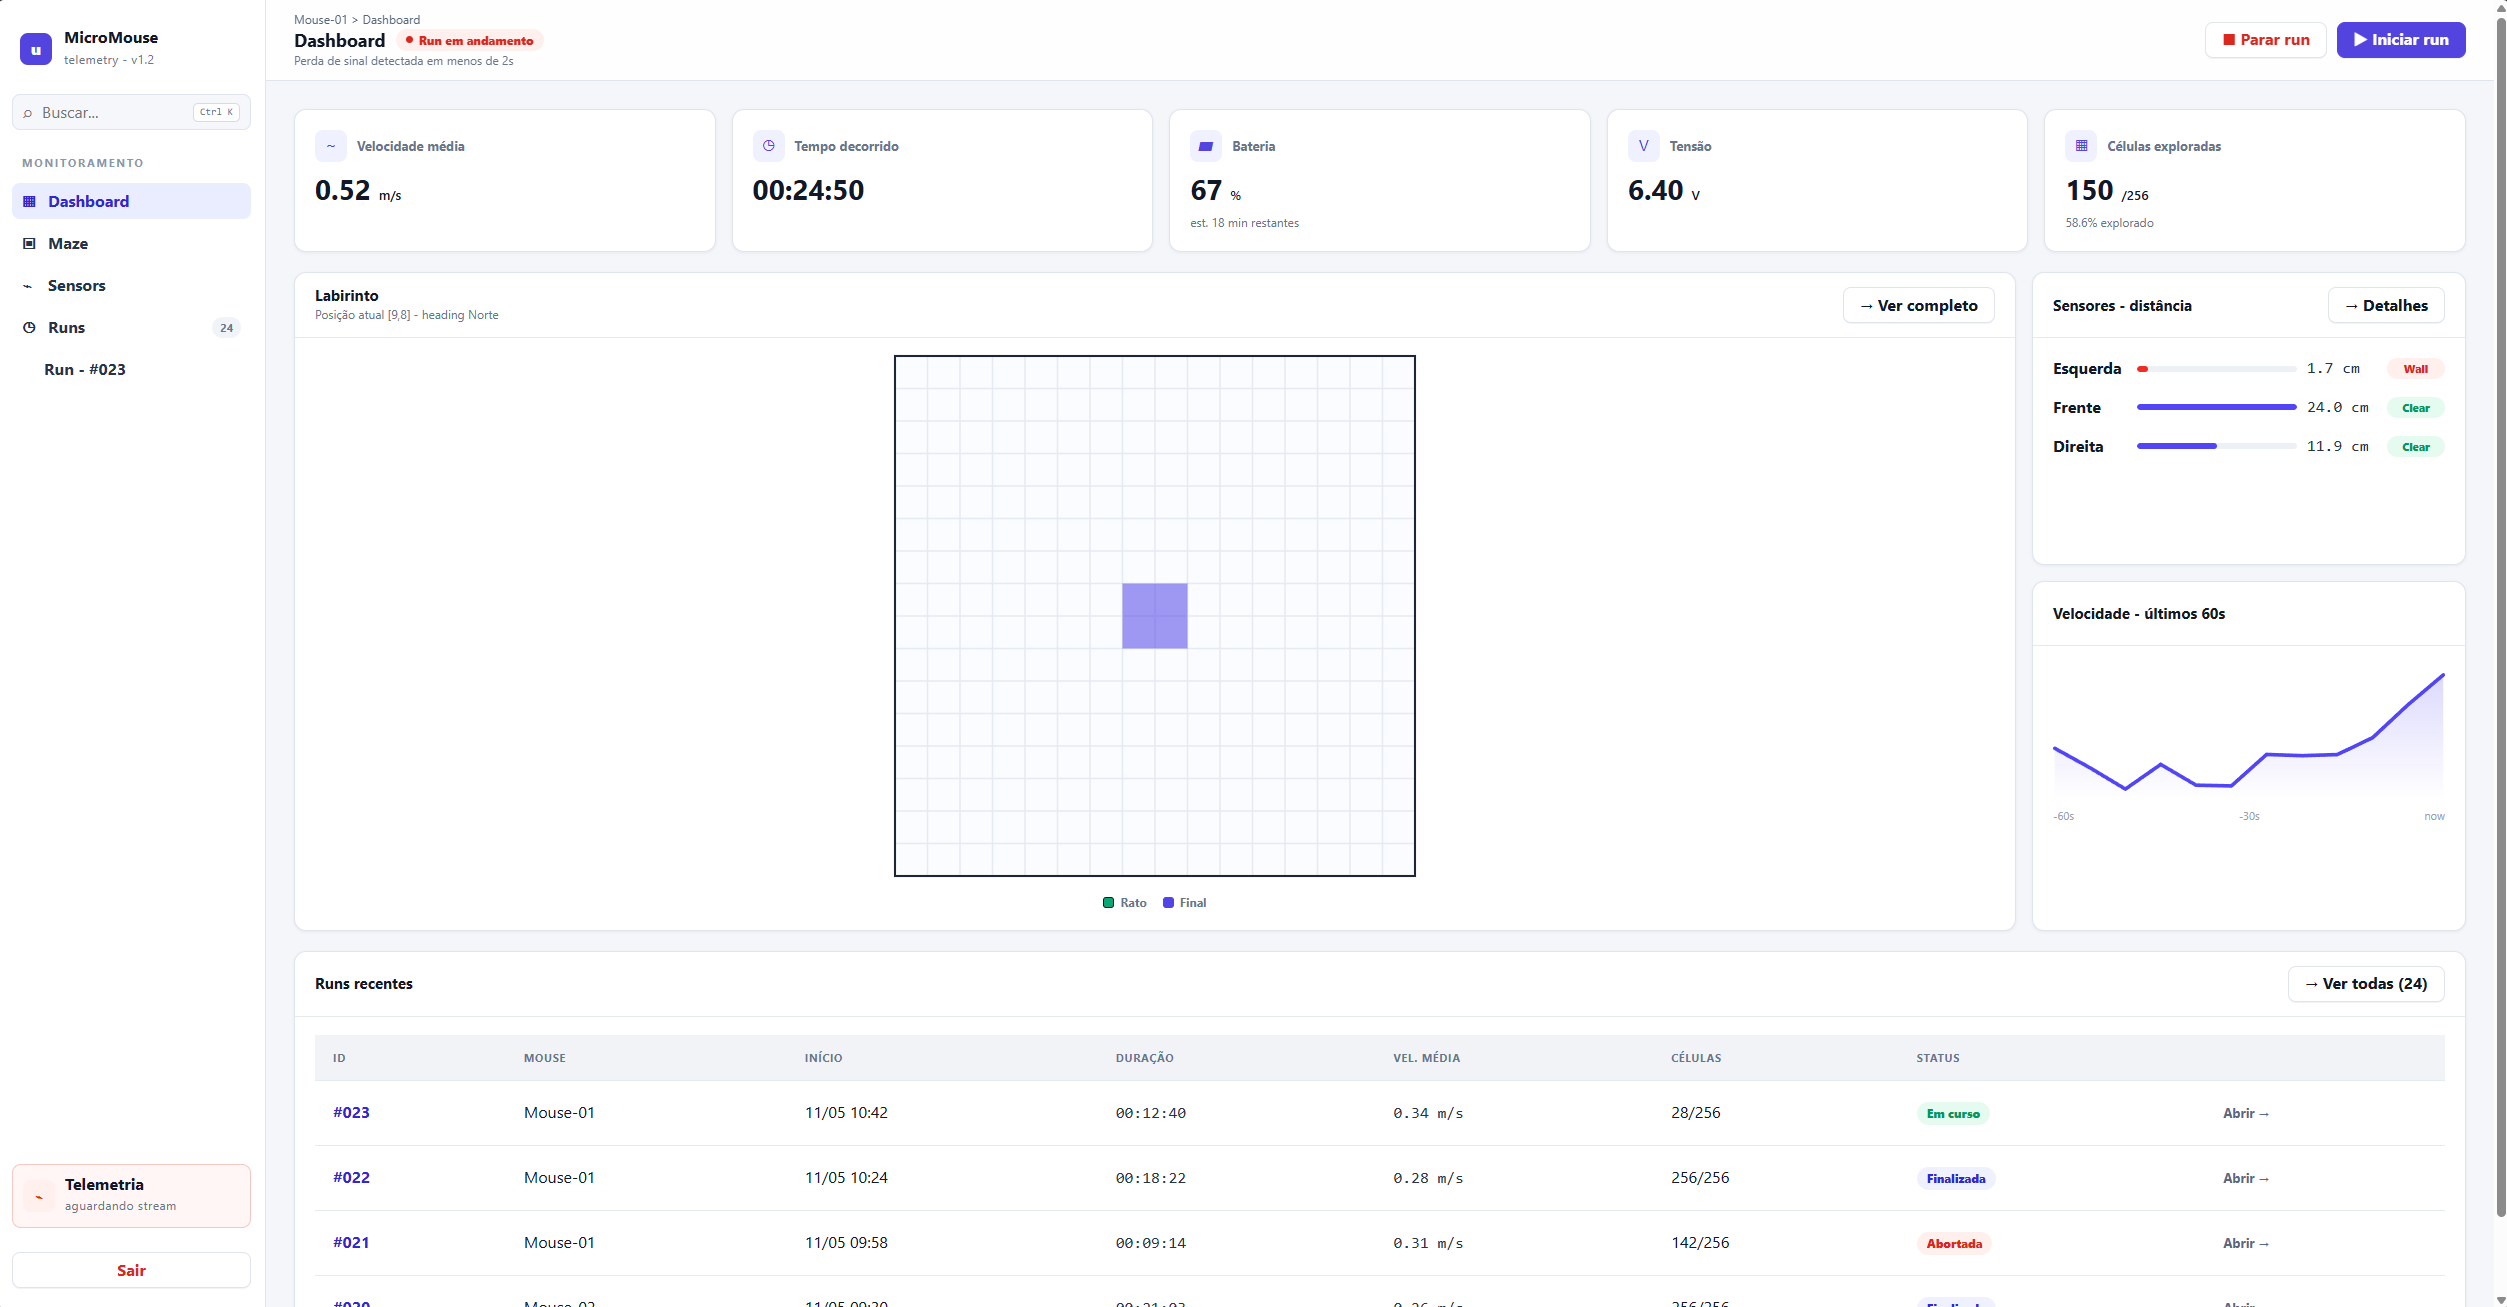
\includegraphics[width=\linewidth]{figuras/dashboard_telemetria_processo.png}
        \caption{Após 25 min: 150 células (58,6\%), bateria 67\%, 6,40~V.}
    \end{subfigure}
    \caption{\textit{Dashboard} de telemetria em dois momentos da corrida simulada.}
    \label{fig:dashboard_telemetria}
\end{figure}

Uma tela dedicada de sensores (Figura~\ref{fig:sensors_telemetria}) exibe o valor atual e o histórico de 60 segundos de cada sensor de distância, um histograma combinado das leituras, o painel de IMU (\textit{roll}, \textit{pitch}, \textit{yaw} e \textit{bias}) e um \textit{stream} de eventos com \textit{timestamps} e velocidades, permitindo verificar a regularidade da chegada dos dados.

\begin{figure}[H]
    \centering
    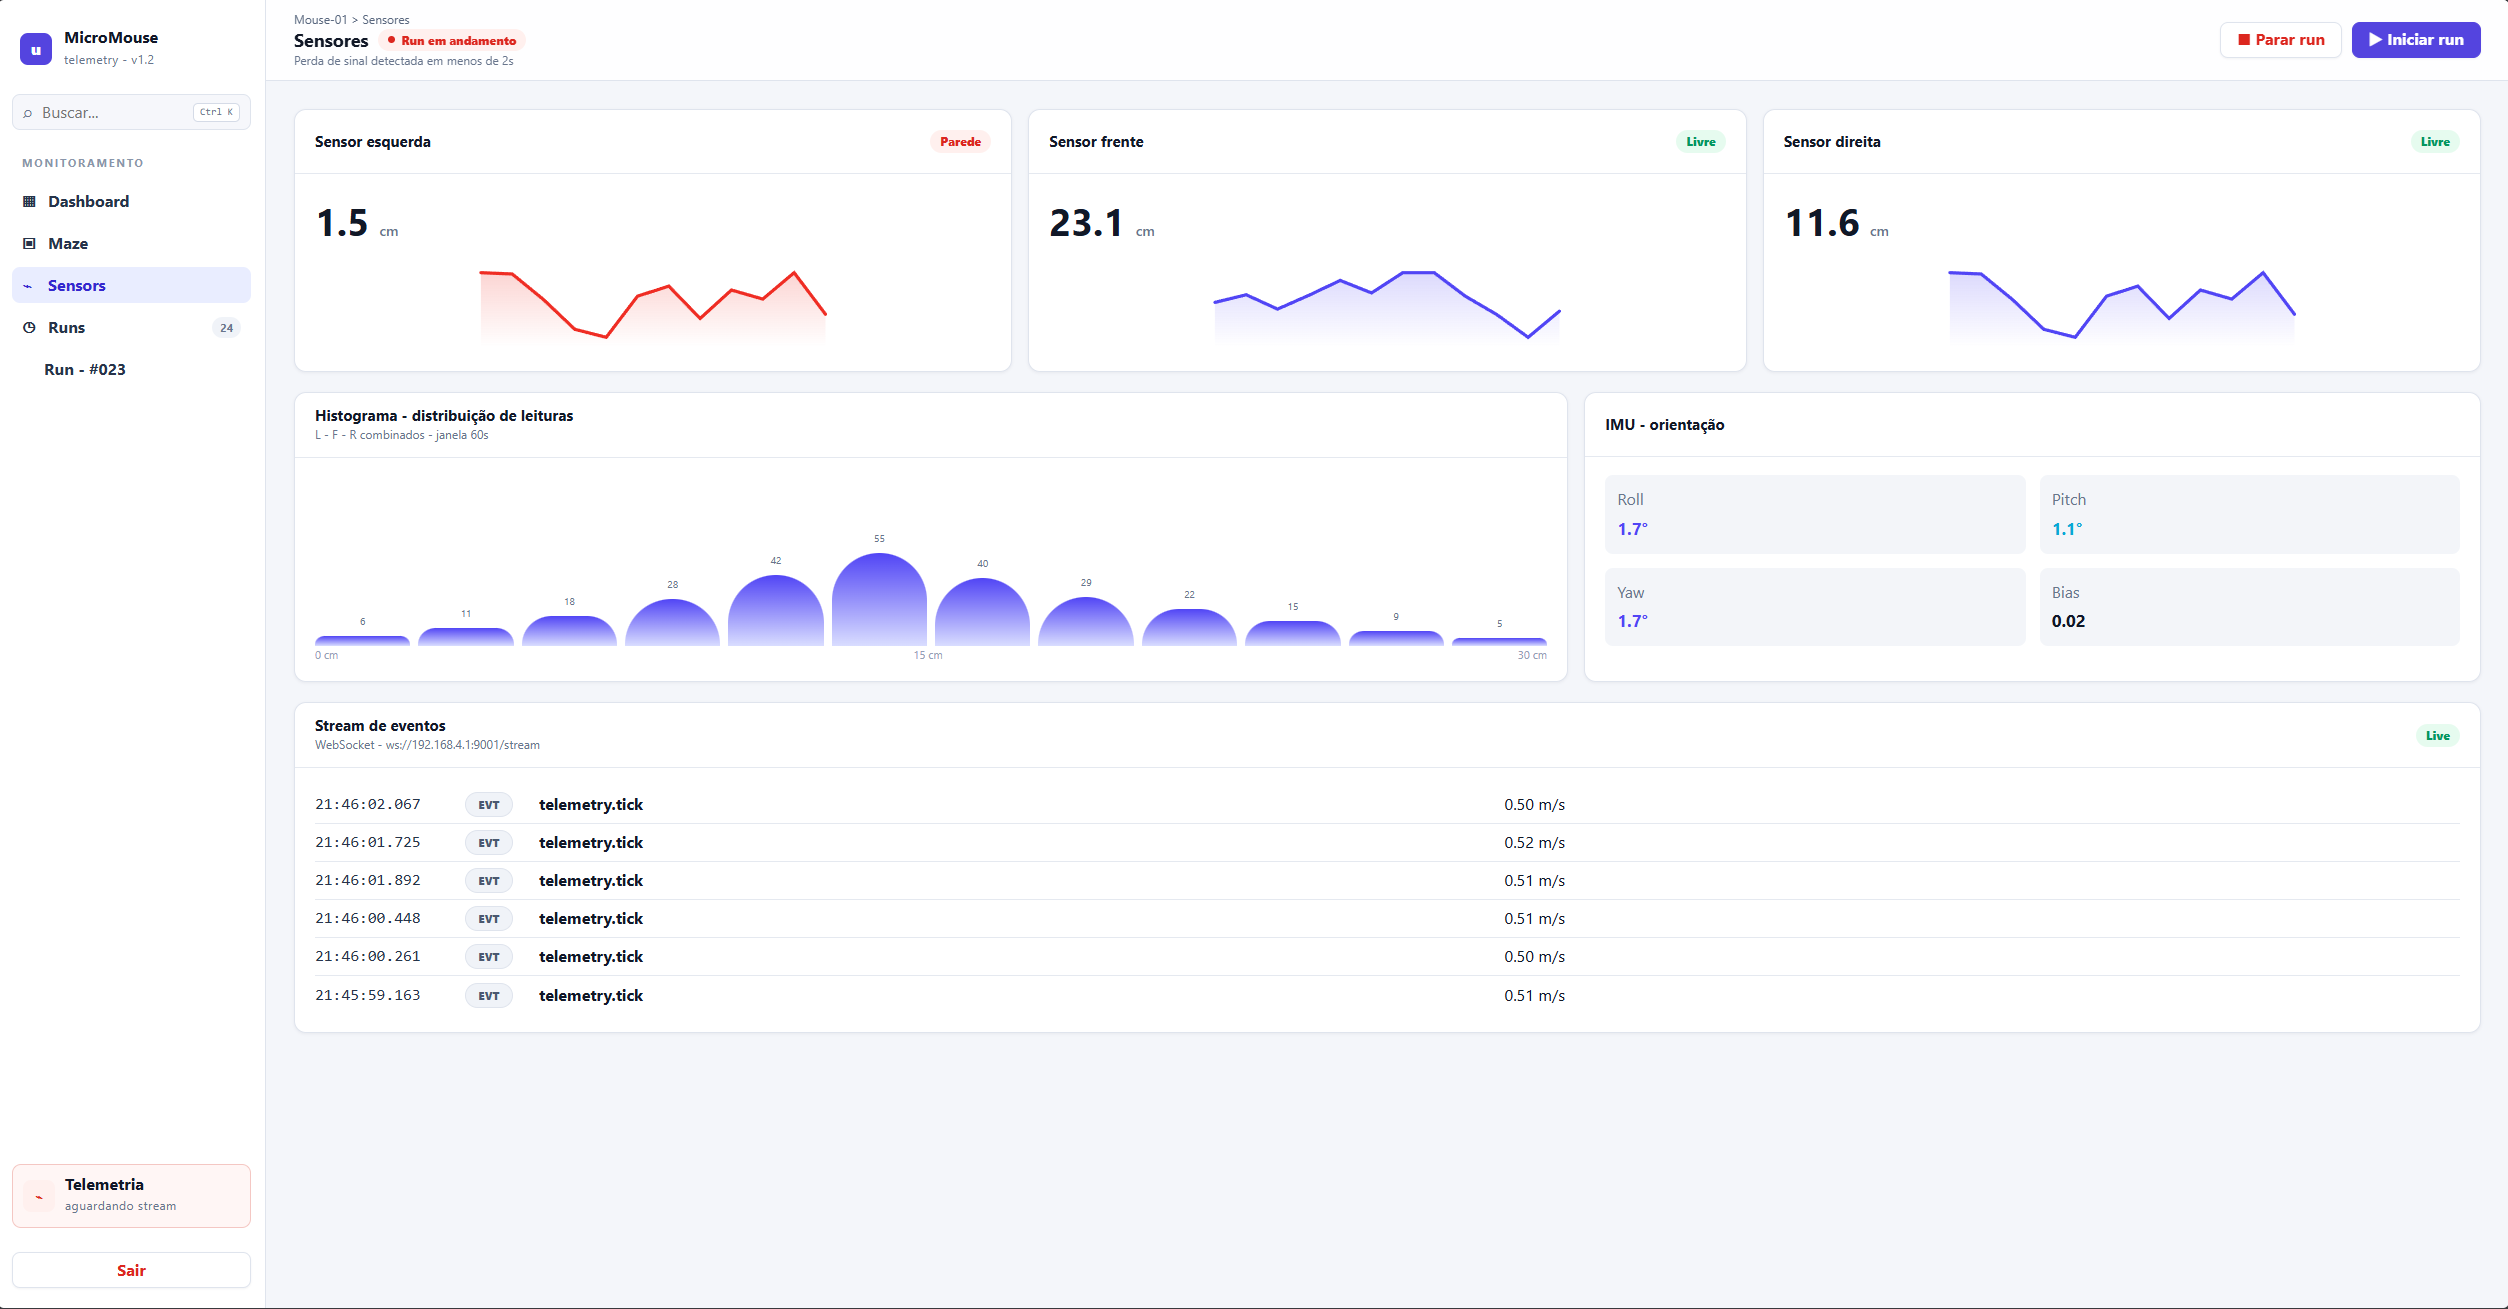
\includegraphics[width=0.85\linewidth]{figuras/sensors_telemetria.png}
    \caption{Tela de sensores durante a corrida simulada: sensor esquerdo detectando parede a 1,5~cm, frente livre a 23,1~cm, direita livre a 11,6~cm, orientação IMU com \textit{roll}/\textit{yaw} de 1,7°.}
    \label{fig:sensors_telemetria}
\end{figure}

\subsection{Mapeamento do labirinto}

O mapa é construído de forma incremental: a cada pacote, o sistema incorpora apenas as células novas ao estado acumulado, armazenado como um JSON esparso no modelo da tentativa. No \textit{frontend}, a grade 16$\times$16 é preenchida à medida que o robô avança; entre os dois registros da Figura~\ref{fig:dashboard_telemetria}, o número de células exploradas saltou de 29 para 150, cobrindo mais da metade do labirinto.

\subsection{Salvamento do caminho percorrido}

Cada passo é salvo individualmente com coordenadas, \textit{timestamp}, orientação, velocidade e bateria, em ordem sequencial que permite reconstruir a trajetória completa. A tentativa em si guarda um resumo -- horário de início e fim, velocidade média, consumo de bateria, status e se o objetivo foi alcançado -- para consulta histórica e análise de desempenho entre corridas.

\subsection{Testes Unitários}

Os testes automatizados do \textit{backend} foram desenvolvidos com Pytest (\texttt{make test}) e alcançaram 90,66\% de cobertura de código (Figura~\ref{fig:figuras/testes_soft.png}), validando a maior parte das funcionalidades implementadas.

\begin{figure}[H]
    \centering
    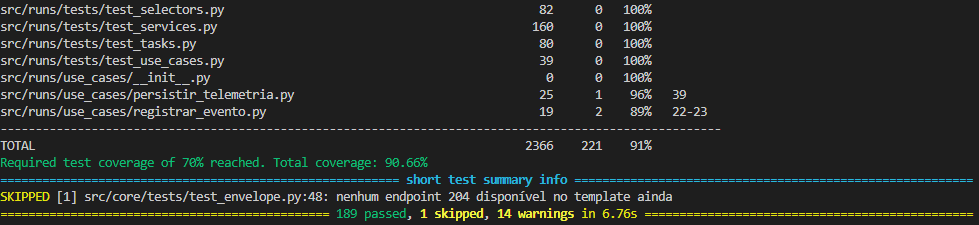
\includegraphics[width=0.7\linewidth]{figuras/testes_soft.png}
    \caption{Coverage de Testes Unitários}
    \label{fig:figuras/testes_soft.png}
\end{figure}

\section{Testes de integração}

A equipe não conseguiu realizar os testes de integração dentro do prazo do Ponto de Controle 2 devido ao atraso na entrega das peças e aos problemas que ocasionaram atrasos na impressão do chassi.

%\textcolor{red}{Apresentar com detalhes os testes feitos para conferir se os objetivos do projeto como um todo foram atendidos.}

%\textcolor{red}{Com relação ao \textit{software}, será necessário apresentar pacotes de componentes de \textit{software}, suas funções e características, e explicar as decisões de projeto.}

